%!TEX root = ../diplom.tex

\section{Моделирование процесса измерения}

Важным преимуществом орбитального радиовысотомера по сравнению с другими
радиолокаторами является то, что теоретические модели рассеяния хорошо
описывают свойства радиолокационного сигнала, отраженного морской поверхностью.
В результате алгоритмы обработки получены не с помощью регрессионного анализа,
а основаны на аналитических формулах для формы отраженного импульса.

Если, например, говорить об определении скорости ветра по сечению обратного
рассеяния для скаттерометра, то алгоритмы были получены благодаря применению
регрессионного анализа массива данных, сформированного из контактных измерений
скорости и направления ветра (морские буи) и сечения обратного рассеяния,
измеренного радиолокатором. Погрешность оценки (не измерения!) скорости ветра
по сечению обратного рассеяния обусловлена неоднозначностью связи скорости
ветра и сечения обратного рассеяния.

У радиовысотомера при определении с высоты значительного волнения происходит
именно процесс измерения, т.к. существует однозначная связь формы переднего
фронта отраженного импульса и высоты значительного волнения, которая выражается
через известную формулу. В данном точность измерения ограничивается параметрами
радиолокатора, в частности, длительностью излучаемого импульса и частотой
дискретизации.

При измерении расстояния от радиолокатора до среднего уровня морской
поверхности алгоритм также опирается аналитические формулы и модели, например,
учитывает особенности распространения электромагнитного излучения в атмосфере и
ионосфере, что позволяет обеспечить высокую точность.

Благодаря возможности достоверного теоретического  описания рассеяния
электромагнитного излучения взволнованной водной поверхностью, численное
моделирование является эффективным инструментом для моделирования работы
радиовысотомера и отладки алгоритмов обработки. С его помощью можно провести
численный эксперимент и рассмотреть по отдельности и в комплексе влияние
множества факторов, которые влияют на точность измерений.

\subsection{Схема измерения}%
\label{sub:skhema_izmereniia}

Преимущество численного моделирования по сравнению с экспериментом состоит в
том, что достаточно просто провести сравнение различных схем измерения и
оценить их эффективность для решения конкретной задачи. Однако для этого
необходимо подробно описать и перевести в числовую форму все важные для
моделирования параметры схемы измерения. В результате это позволит провести
полноценный <<численный>> эксперимент.  Для описания схемы измерения необходимо
задать угол зондирования (падения) $\theta_0$, высоту орбиты $H_0$, скорость и
направление движения $v_{rad}$, и направление зондирования $\phi_{rad}$. На рис.\ref{fig:geometry} показана схема измерения. 

Расстояние от радиолокатора до точки отражения на плоскости $xy$ равно $R_0$ .
Для определенности выберем направление движения радиовысотомера вдоль оси $x$.


Для плоской поверхности формирование отраженного импульса начинается при
касании поверхности передним фронтом падающего импульса в точке непосредственно
под радиовысотомером. Это кратчайшее расстояние от радиовысотомера до
поверхности. На рис.\ref{fig:wave_form} показан пример изменения формы
рассеивающей площадки и формы отраженного импульса в зависимости от времени.
\begin{figure}[h]
    \centering
    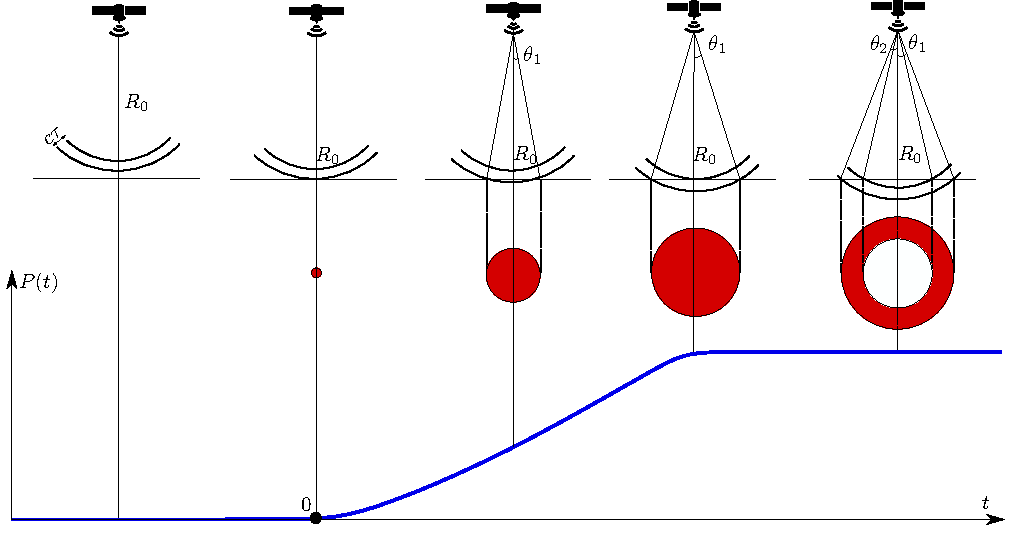
\includegraphics[]{fig/flat_wave1.pdf}
    \caption{}
    \label{fig:}
\end{figure}

\begin{figure}[h]
    \centering
    \hfill
    \begin{subfigure}{0.25\linewidth}
        \centering
        \includesvg{wave_front2}
    \end{subfigure}
    \hfill
    \begin{subfigure}{0.25\linewidth}
        \centering
        \includesvg{wave_front3}
    \end{subfigure}
    \hfill
    \begin{subfigure}{0.25\linewidth}
        \centering
        \includesvg{wave_front4}
    \end{subfigure}
    \label{fig:wave_form}
    \caption{Геометрическая интерпретация формы отраженного импульса}
\end{figure}

Для нахождения отраженного имульса необходимо выполнить интегрирование по
рассеивающей площадке для сферической волны с учетом длительности зондирующегоо
импульса.


%\subsection{Влияние морского волнения на форму отраженного импульса}%
%\label{sub:vliianie_morskogo_volneniia_na_vormu_otrazhennogo_impul_sa}

Если говорить о морской поверхности, то перед интегрированием по рассеивающей
площадке необходимо выяснить какие участки поверхности будут вносить свой вклад
в формирование отраженного импульса.  При малых углах падения механизм обратного  рассеяния является квазизеркальным и отражение происходит на участках волнового профиля, ориентированных
перпендикулярно падающему излучению. Тогда в формировании отраженного сигнала
будут участвовать только площадки, ориентированные нормально к излучению. 
Поэтому для моделирования рассеяния нам необходимо знать не только высоту
в выбранной точке точке, но и уравнение касательной к ней плоскости, другими словами необходимо знать наклоны $\zeta_x$ и  $\zeta_y$ в искомой точке.

%\footnote{Под словосочетанием <<отражающая точка>> подразумевается
    %физически малая отражающая площадка с большим радиусом кривизны, по которой
%во время вычисления отраженного поля производится интегрирование}. 

Зная координаты радиолокатора  $(x_0,y_0,z_0)$, координаты точки на
поверхности $(x,y,z)$ и наклоны в этой точке $(\zeta_x,\sigma_y,1)$, можем из
геометрии (см. рис. \ref{fig:local_theta}) получить локальный угол падения
излучения $\theta_0$:
\begin{equation}
    \label{eq:local_theta}
    \cos \theta =  \frac{\vec R \vec n}{|\vec R| |\vec n|}, \text{ где}
\end{equation}
$R$ -- расстояние от радиолокатора до отражающей точки точки,
 $\vec n$ -- нормально касательной плоскости, проведенной к отражающей точке.
 В случае численного моделирования, когда мы хотим решить задачу нахождения
 формы отраженного импульса от известной морской поверхности, можем найти
 $\vec R$ как
 \begin{equation}
     \label{eq:R_1}
     \vec R = \vec R_0 + \zeta_x \vec n_z,
 \end{equation}




Вероятность того, что угол $\theta_0$ будет точно равен нулю и произойдет
зеркальное отражение для случайной выбранной точки очень мала, поэтому имеет
смысл рассматривать квазизеркальное отражение и вводить ограничение на
максимально допустимый локальный угол отражения. 

Нахождение всех зеркальных точек на характерном пятне радиолокатора  $5\times
5 \text{ км}^2$ представляет собой ресурсоемкую задачу. Но поскольку формирование
импульса носит статистический характер, то мы можем ограничится лишь выборкой зеркальных точек. 

%Процесс создания такой выборки продемонстрирован на рис.
%\ref{fig:mirror:a}-\ref{fig:mirror:c}. 
%Реализация процесса создания выборки и интегрирования по рассеивающим
%площадкам, входящим в неё представлена в листинге \ref{lst:pulse}.

%Для смоделированной поверхности  рис. \ref{fig:mirror:a} вычисляются по формуле \eqref{eq:local_theta} локальные углы
%падения $\theta_0$. Если локальный угол падения оказывается меньше некоторой
%наперед заданной точности\footnote{эмпирическим путем выяснилось, что отклонение
%$\theta_0$ от нуля не более чем на $1^\circ$ является допустимым}, то точка падения в дальнейшем
%считается зеркальной, а значит вносящей вклад в формирование отраженного
%импульса. 
%Выборку можно делать несколькими способами, например создать её выбирая случайные точки на координатной сетке или проходить
%координатную сетку с равномерным шагом. 
%Выборка на рис. \ref{fig:mirror:b} и \ref{fig:mirror:c} получена вторым
%способом. 



\begin{figure}[h!]
    \centering
    \def\svgwidth{0.75\linewidth}
    \includesvg{local_theta}
    \caption{Геометрия определения локального угла падения. Красной линией
    обозначена касательная плоскость к рассматриваемой отражающей точке
$(x,y,\zeta)$}
    \label{fig:local_theta}
\end{figure}

\begin{figure}[h!]
    \centering
    \begin{subfigure}{0.65\linewidth}
        \centering
        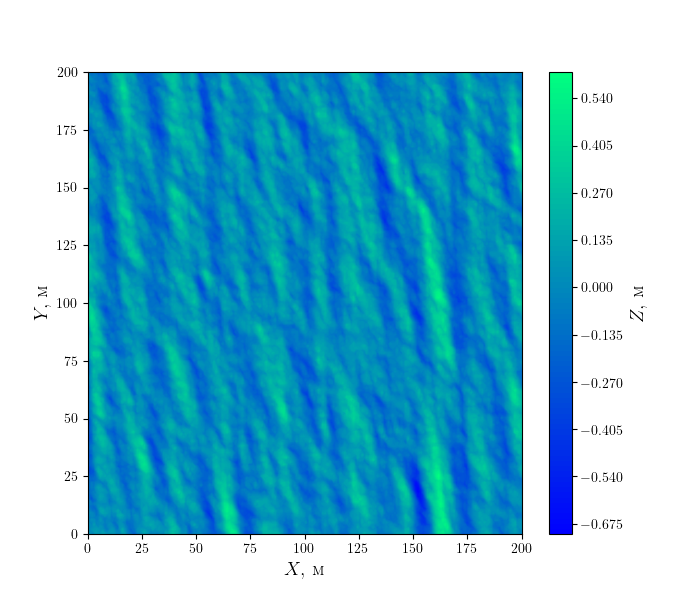
\includegraphics[width=\linewidth]{fig/impulse/fig1}
        \caption{Моделирование поверхности при скорости ветра $U=5$ м/с}
        \label{fig:mirror:a}
    \end{subfigure}
    \begin{subfigure}{.49\linewidth}
        \centering
        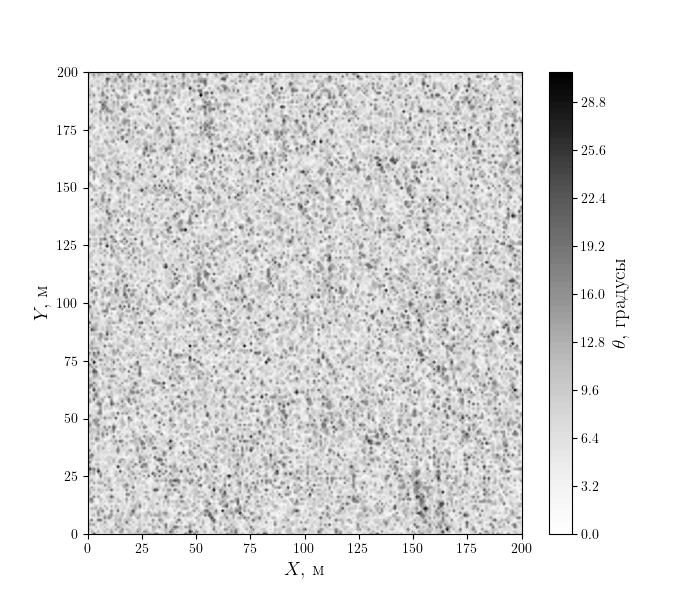
\includegraphics[width=\linewidth]{fig/impulse/fig2}
        \caption{Локальный угол отражения от поверхности для радиолокатора
        находящегося на высоте $H=1000$ км в точке с координатой (100, 100)}
        \label{fig:mirror:b}
    \end{subfigure}
    \begin{subfigure}{.49\linewidth}
        \centering
        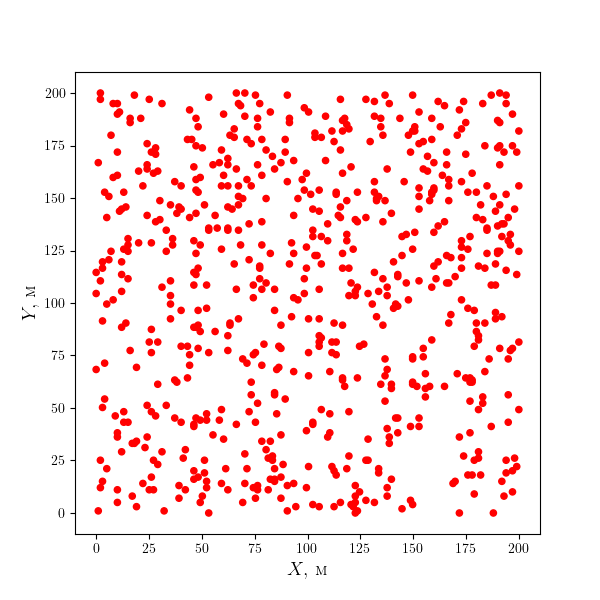
\includegraphics[width=\linewidth]{fig/impulse/fig3}
        \caption{Положение зеркальных точек поверхности \ref{fig:mirror:a} для
        радиолокатора находящегося над точкой (100,100) }
        \label{fig:mirror:c}
    \end{subfigure}
    \label{fig:mirror}
    \caption{}
\end{figure}

Теперь, для вычисления поля вблизи приемной антенны радиолокатора нам
необходимо просуммировать отраженное от квазизеркальных точек поле
(см.рис. \ref{fig:mirror:c}).  


%Как было сказано с предыдущих разделах, волна излученная антенной
%является сферической, а значит её амплитуда  спадает по гиперболическому закону. Тогда амплитуда поля вблизи точки отражения
%$(x,y,\zeta)$
%будет определяться как (см. геометрию задачи на рис. \ref{fig:local_theta})
Запишем скалярное поле, излучаемое антенной радиолокатора в зеркальную точку с радиус-вектором $\vec
R$
\begin{equation}
    \label{eq:}
    E_{s}(\vec R,t) = \frac{E_0}{R}  \cdot  e^{i(\omega t - \vec k \vec
    R)} U(t)G(\theta), 
\end{equation}
где $U(t)$ -- некотораря функция, ограничивающая длительность импульса,
$G(\theta)$ -- диаграмма направленности антенны.

Тогда вблизи приемной антенны амплитуду поля $E$ можно записать как
\begin{equation}
    \label{eq:E}
    E \sim \frac{E_{sur}}{R_1} e^{-i\vec k \vec R} \cdot G(\theta) =
    \frac{E_0}{R^2} e^{-2i\vec k \vec R} \cdot G^2(\theta), 
\end{equation}

Остается только проинтегрировать уравнение \eqref{eq:E} по всем отражающим
точкам 

\begin{equation}
    \label{eq:}
    E \sim \sum\limits_{i=1}^{M} \frac{E_0}{R_i^2} \exp{-2ikR_i}
    G^2(x,y,\theta_0)
\end{equation}
где $M$ -- количество точек,  $x_i,y_i$ -- координаты  $i-$ой отражающей точки,
 $R_i$-- расстояние от спутника до  $i-$ой точки.

 \textbf{\color{red} {\large Вопрос. Как должно выглядеть <<честное>> выражение
 для амплитуды поля? Верно понимаю, что там нужно ещё только дописать УЭПР
 площадки и умножить на площадь площадки? То есть}
\begin{equation}
    \label{eq:}
    E =  \sum\limits_{i=1}^{M} \frac{E_0}{R_i^2} \exp{-2ikR_i} \sigma^o_i
    \Delta S_i
\end{equation}
 как правильнее в дальнейшем учесть вес каждой точки? Или здесь мы снова
 опираемся на статистические свойства формы импульса и считаем, что площадки
 имеют одинаковый вес? В отчете выдвигало предположение, что они имеют
 одинаковый вес, но потом нигде не рассматривался случай невыполения этого
 предположения}%

 Результирующая мощность импульса будет равна
 \begin{equation}
     \label{eq:}
     P(t) = \frac{EE^*}{2}
 \end{equation}
Процесс создания такой выборки зеркальных точек продемонстрирован на рис.
\ref{fig:mirror:a}-\ref{fig:mirror:c}. 
Реализация процесса создания выборки и интегрирования по рассеивающим
площадкам, входящим в неё представлена в листинге \ref{lst:pulse}.
На рис. \ref{fig:model_pulse} представлен импульс, посчитанный суммированием по отражающим точкам.

 \begin{figure}[h]
     \begin{subfigure}{.59\linewidth}
         \centering
         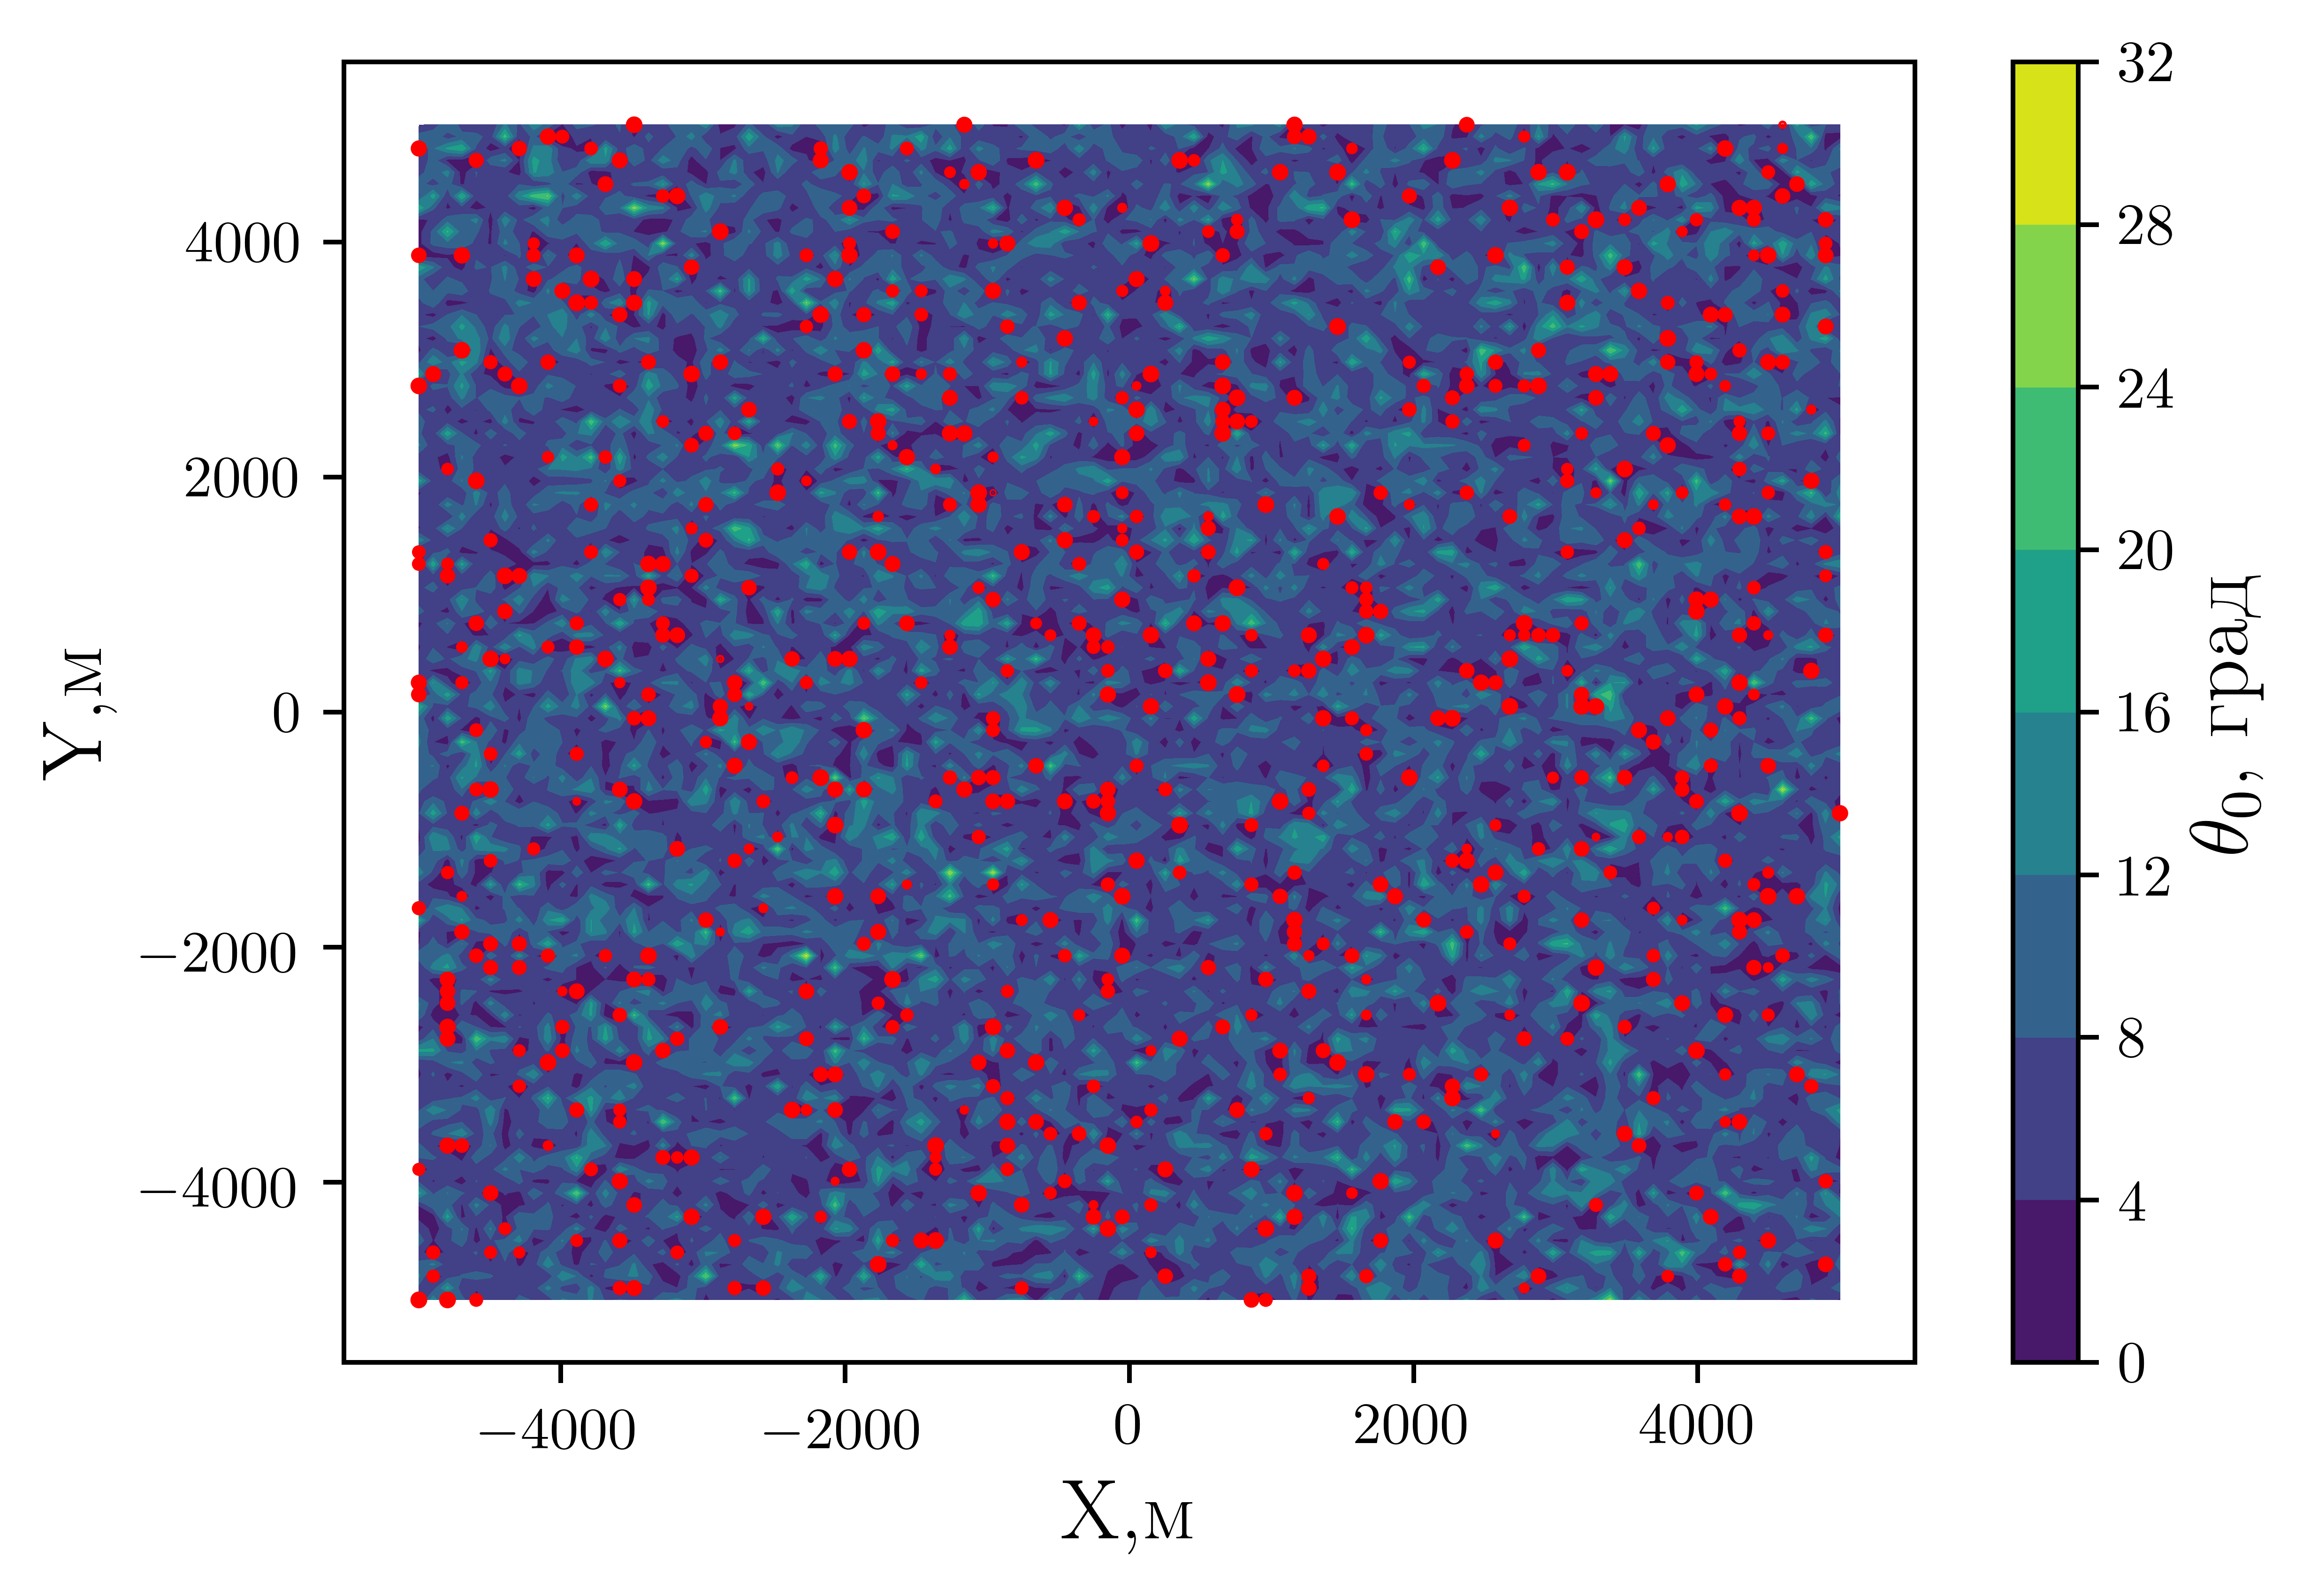
\includegraphics[width=\linewidth]{fig/model_mirrors1}
         \caption{}
     \end{subfigure}
     \begin{subfigure}{.39\linewidth}
         \centering
         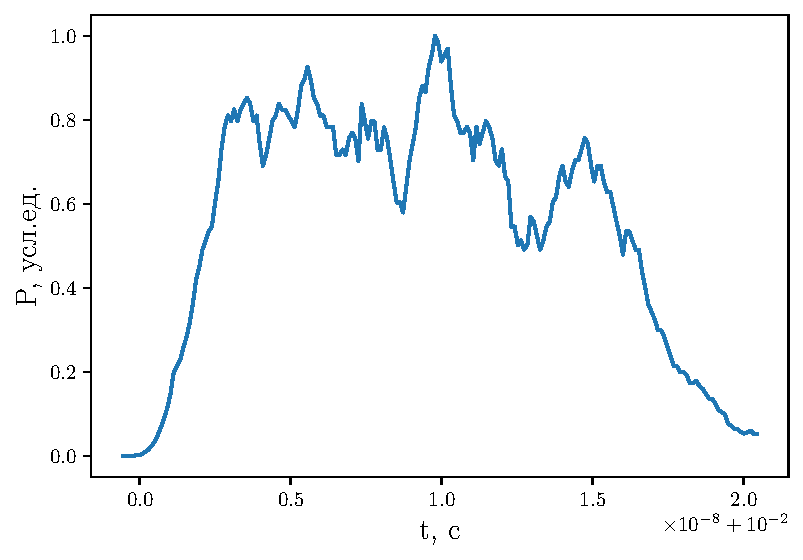
\includegraphics[width=\linewidth]{fig/model_impuls1}
         \caption{}
     \end{subfigure}
     \caption{(a) Вычисление локального угла падения (см.\eqref{eq:local_theta} )для радиолокаторе,
     находящегося в точке $(0,0,h)$. Красным цветом обозначены точки, которые в
 дальнейшем будут считаться зеркальными и которые будут участвовать в
 формировании отраженного импульса.
 (b) Мощность отраженного импульса в зависимости от времени.}
    \label{fig:model_impuls}
 \end{figure}





 \textbf{\color{red} \large Вопрос. Как получить форму импульса, соответствующую
 формуле Брауна?}%
 { \color{red}
 На самом деле график на рис. \ref{fig:model_impuls}b похож на формулу Брауна,
 но очень сильно зашумленную (просматривается передний фронт, задний тоже можно
 найти, если иметь хорошее воображение). 
 Насколько я понимаю, для этого мне необходимо производить измерения с помощью
 не единичного импульса, а их серии (я всё же начинал обрабатывать данные
 присланные Ростовом и видел, что на реальные радиолокаторы производят порядка
 сотни импульсов). Должен ли я теперь моделировать несколько импульсов, но с
 учетом эволюции морской поверхности? Сделал бы это сразу, но такой численный
 эксперимент требует больших вычислительных затрат, из-за необходимости
 моделирования сразу нескольких морских поверхностей, поэтому решил спросить у
 вас и перестраховаться.}

 {\color{red} Ниже представлены на рис. \ref{fig:flat_surf} графики моделирования получения импульса, отраженного от
плоской поверхности. Насколько я понимаю, шумы в такой простой задаче вызваны
когерентным суммированием гармоник на приемной антенне. А спадание импульса
вызвано особенностями моделирования: при распространении сферической волны в
плоскости $xy$ она выходит за границы рассматриваемой координатной сетки, тем
самым уменьшая количество зеркальных точек, а значит и уменьшая мощность в
результате. В этом можно убедиться, если увеличить координатную сетку.
Например, на рис. \ref{fig:flat_surf1} я увеличил немного координатную сетку и
задний фронт действительно дольше не спадал. Получается, чтобы избежать таких
ошибок, необходимо связывать размер кооординатной сетки, на которой ищутся
зеркальные точки с длительность времени, за которое мы можем моделировать
импульс.}




 \begin{figure}[H]
     \begin{subfigure}{.59\linewidth}
         \centering
         \includegraphics[width=\linewidth]{fig/model_mirrors2}
         \caption{}
     \end{subfigure}
     \begin{subfigure}{.39\linewidth}
         \centering
         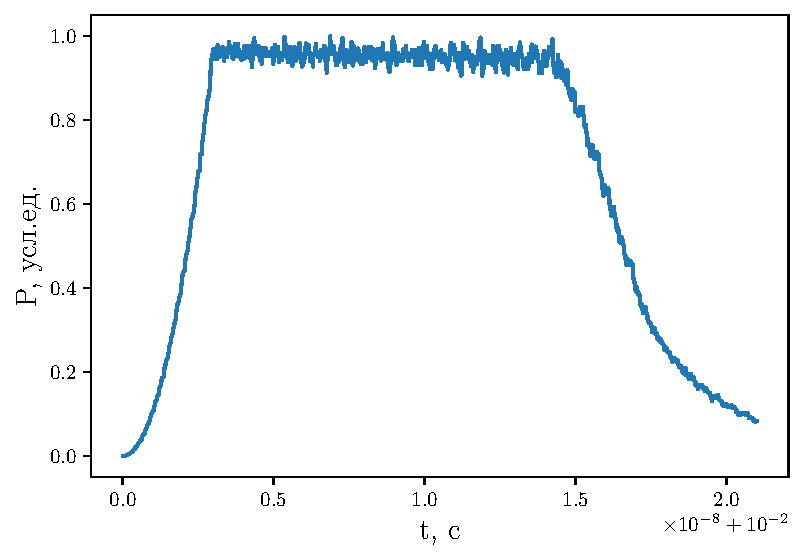
\includegraphics[width=\linewidth]{fig/model_impuls2}
         \caption{}
     \end{subfigure}
     \caption{(a) Вычисление локального угла падения (см.\eqref{eq:local_theta} )для радиолокаторе,
     находящегося в точке $(0,0,h)$. Красным цветом обозначены точки, которые в
 дальнейшем будут считаться зеркальными и которые будут участвовать в
 формировании отраженного импульса.
 (b) Мощность отраженного импульса в зависимости от времени.}
 \label{fig:flat_surf}
 \end{figure}

 \begin{figure}[h]
     \begin{subfigure}{.59\linewidth}
         \centering
         \includegraphics[width=\linewidth]{fig/model_mirrors4}
         \caption{}
     \end{subfigure}
     \begin{subfigure}{.39\linewidth}
         \centering
         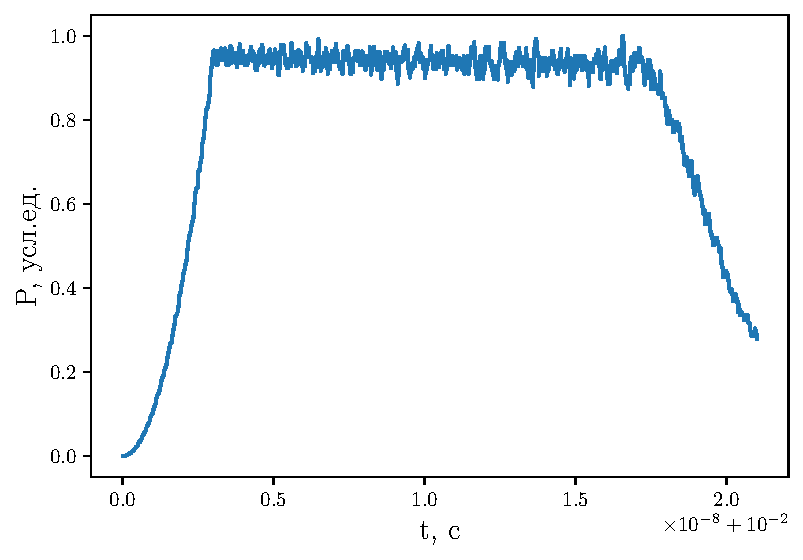
\includegraphics[width=\linewidth]{fig/model_impuls4}
         \caption{}
     \end{subfigure}
     \caption{(a) Вычисление локального угла падения (см.\eqref{eq:local_theta} )для радиолокаторе,
     находящегося в точке $(0,0,h)$. Красным цветом обозначены точки, которые в
 дальнейшем будут считаться зеркальными и которые будут участвовать в
 формировании отраженного импульса.
 (b) Мощность отраженного импульса в зависимости от времени.}
     \label{fig:flat_surf1}
 \end{figure}
 \begin{figure}[H]
     \begin{subfigure}{.59\linewidth}
         \centering
         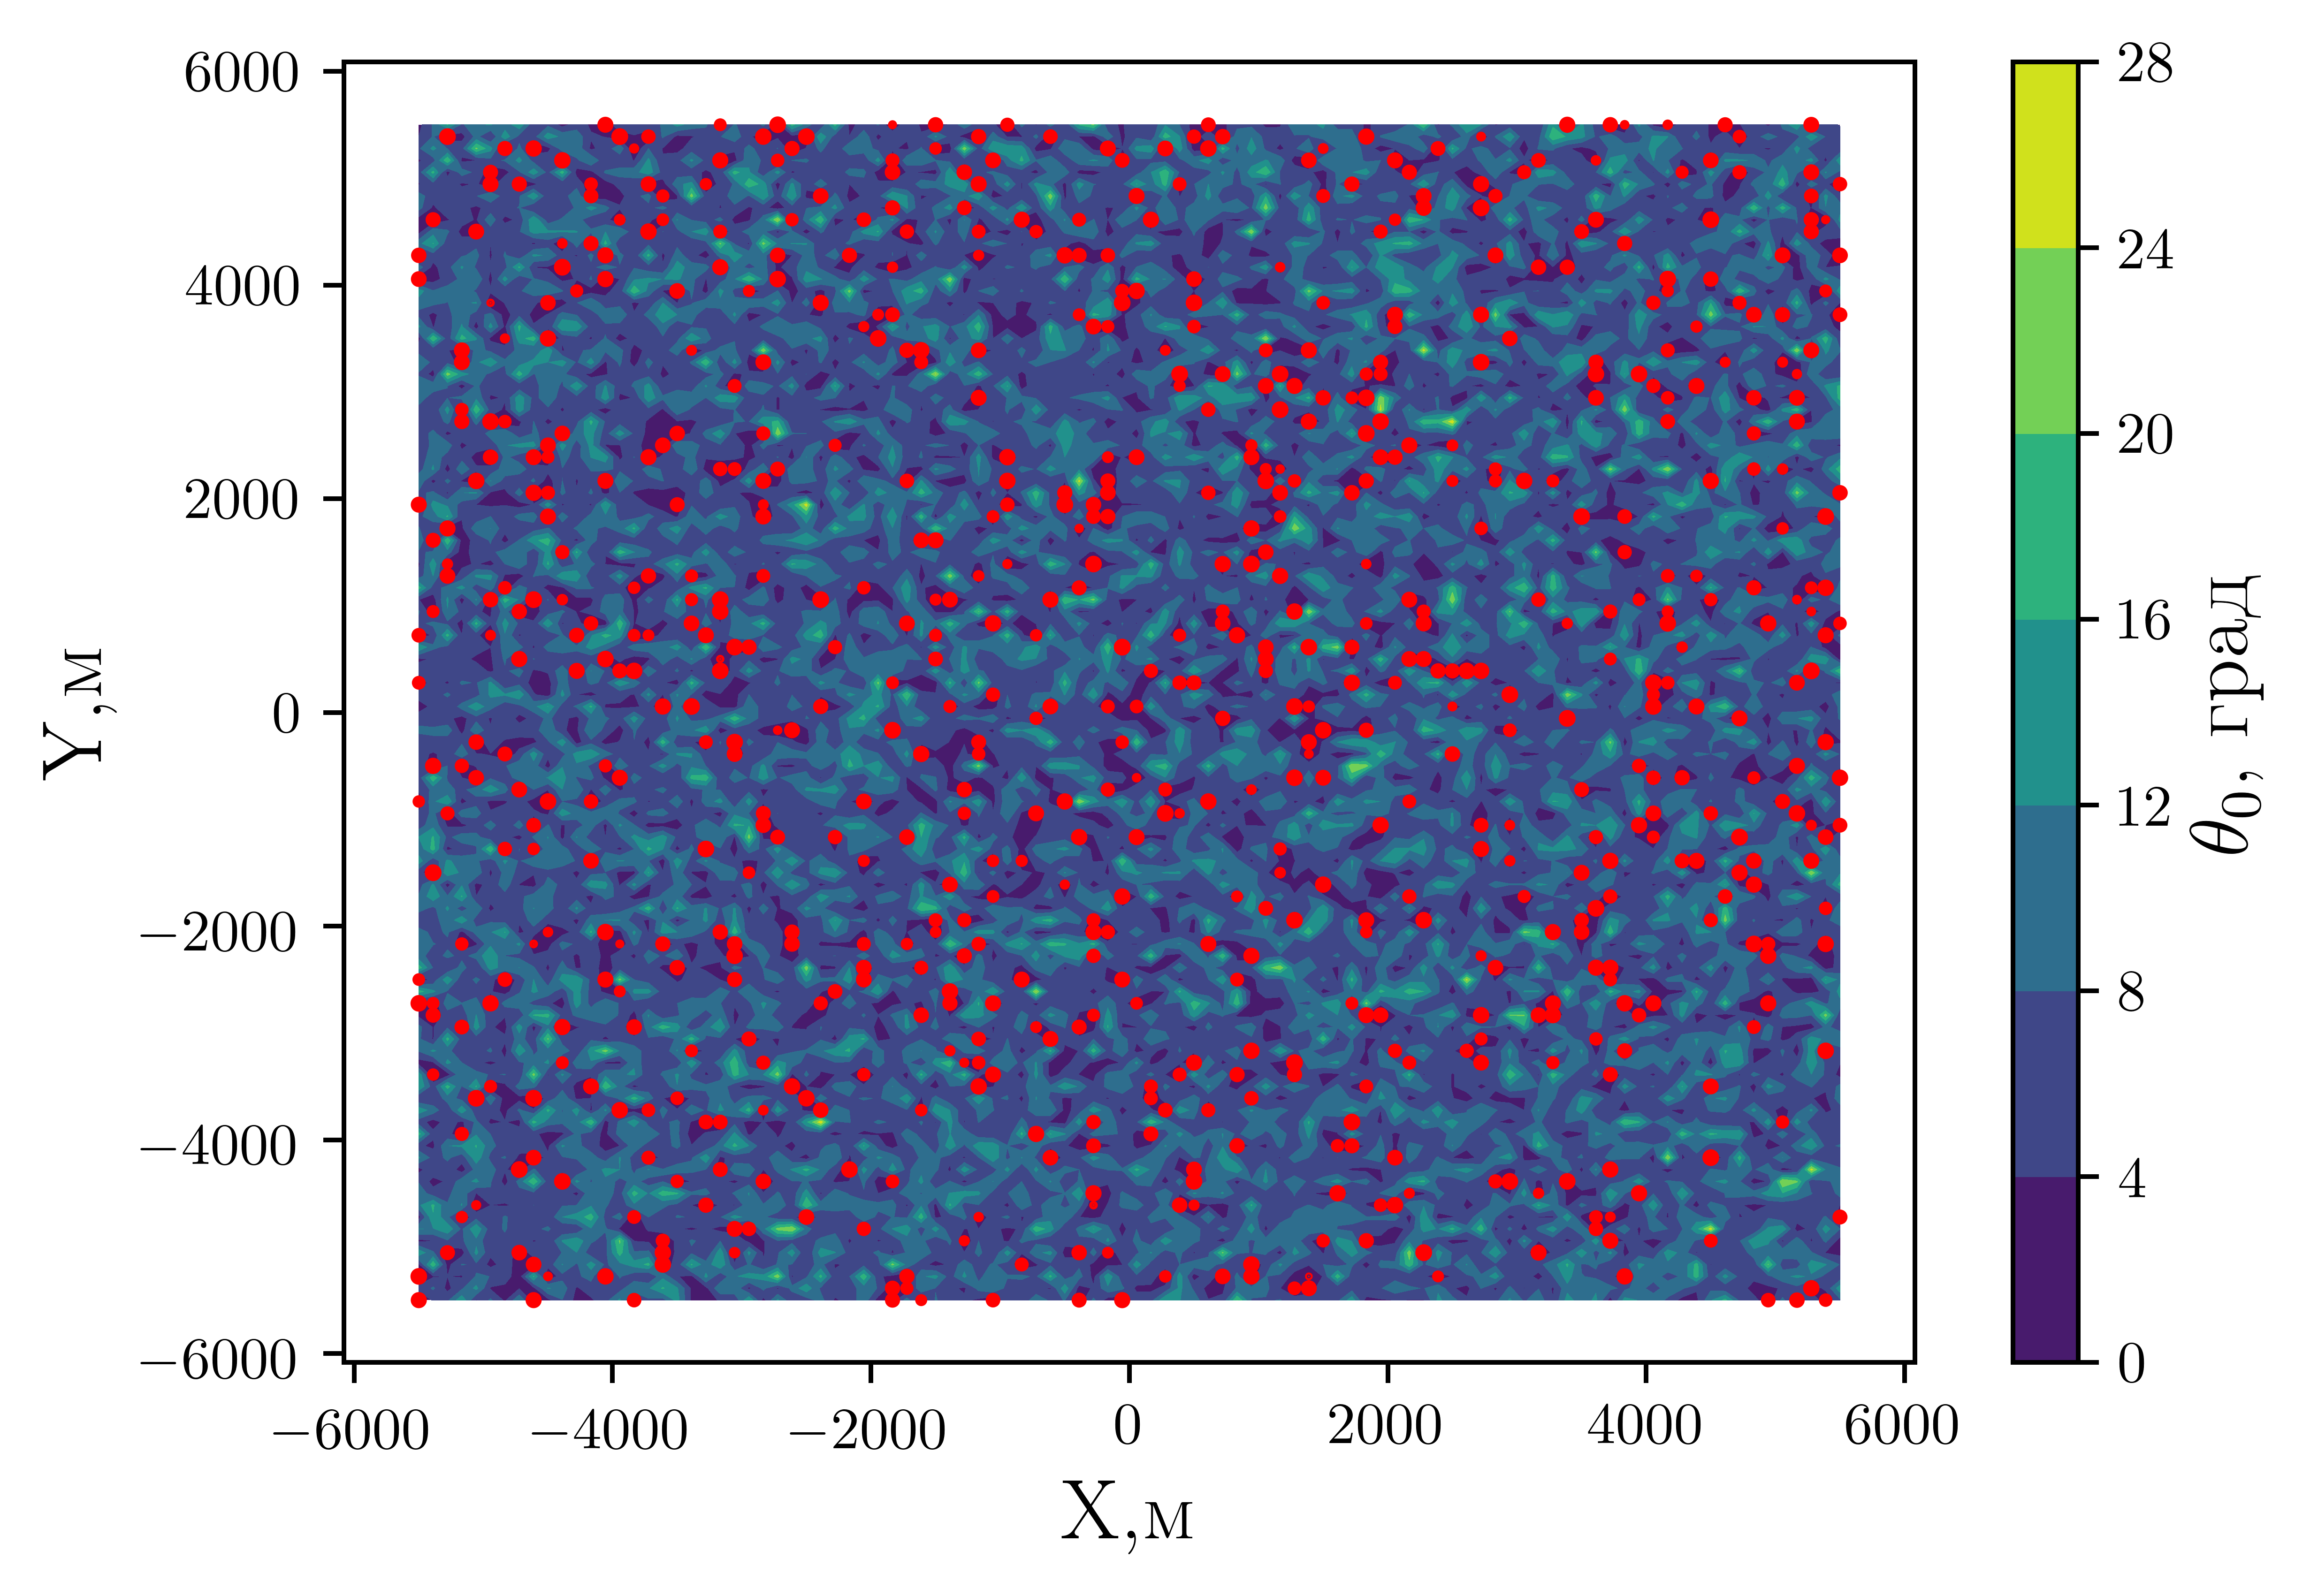
\includegraphics[width=\linewidth]{fig/model_mirrors3}
         \caption{}
     \end{subfigure}
     \begin{subfigure}{.39\linewidth}
         \centering
         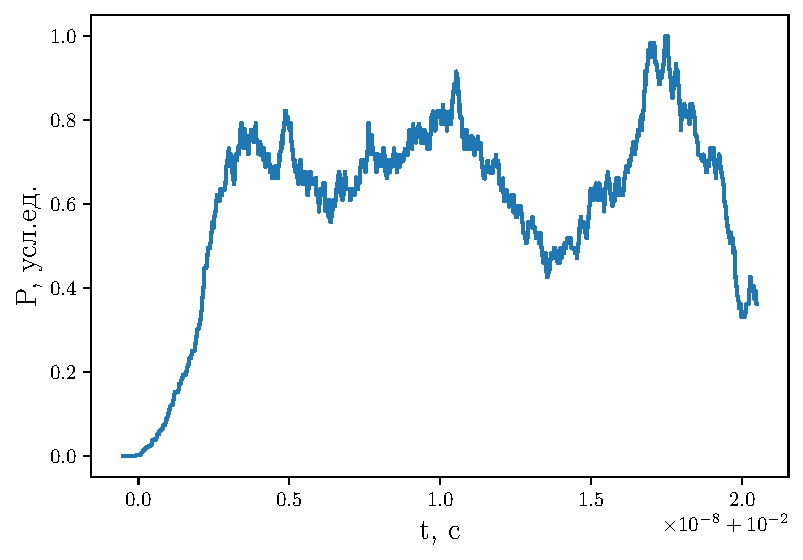
\includegraphics[width=\linewidth]{fig/model_impuls3}
         \caption{}
     \end{subfigure}
     \caption{(a) Вычисление локального угла падения (см.\eqref{eq:local_theta} )для радиолокаторе,
     находящегося в точке $(0,0,h)$. Красным цветом обозначены точки, которые в
 дальнейшем будут считаться зеркальными и которые будут участвовать в
 формировании отраженного импульса.
 (b) Мощность отраженного импульса в зависимости от времени.}
    \label{fig:}
 \end{figure}


\appendix
\newpage
\section{Моделирование отраженного импульса}%
\label{app:sec:pulse}
Весь проект был написан на Python 3.8 с целью облегчить чтение исходного кода.
Также целью было поставлено использование, где это возможно, внешних
высокоптимизированных методов библиотеки NumPy, которая позволяет значительно
упростить и ускорить операции с массивами данных.

Например, для вычисления локального угла падения по формуле
\eqref{eq:local_theta} необходимо реализовать вложенный цикл, который будет
считать значение $\theta$ в каждой точке на выбранной сетке  $(x,y)$. Это,
разумеется, несложно сделать, но все вычисления в этом цикле будут
производиться в один поток. Но современные процессоры могут производить
вычисления в несколько потоков, необходимо лишь правильно написать для этого
код. В Python'е многопоточности можно добиться несколькими путями: вручную
создавать нужное количество потоков для выбранного числа ядер или же
при вычислении использовать библиотеки, в которых это уже реализовано. 
В данном использование метода
\python{np.einsum()} позволило использовать
все 8 потоков компьютера, на котором писался этот отчет, а не один.

Все методы в листинге \ref{lst:pulse} предполагают, что уже выполнено
численное моделирование морской поверхности и оттуда получены массивы с
координатами $\vec r = (x,y,z)$ точек и значениями наклонов $\vec n =
(\zeta_x,\zeta_y,1)$.




\lstinputlisting[caption={Моделирование отраженного
импульса},label={lst:pulse},captionpos=t]{scripts/pulse.py}
